\chapter{分散型分光器}


% 分光器とは光を波長ごとに分けそれぞれの波長での光の強度を測定する装置である.
% 主にスリット,コリメータ,回折格子,結像器,検出器から構成されている.
% 本研究ではコリメータ及び結像器にアクロマティックレンズ,検出器にはCCDカメラを用いる.





\section{ツェルニ・ターナ型分光器}
図\ \ref{fig:czerny_turner}に代表的な分散型分光器であるツェルニ・ターナ型分光器の概略図を示す.
\begin{figure}[htbp]
    \centering
    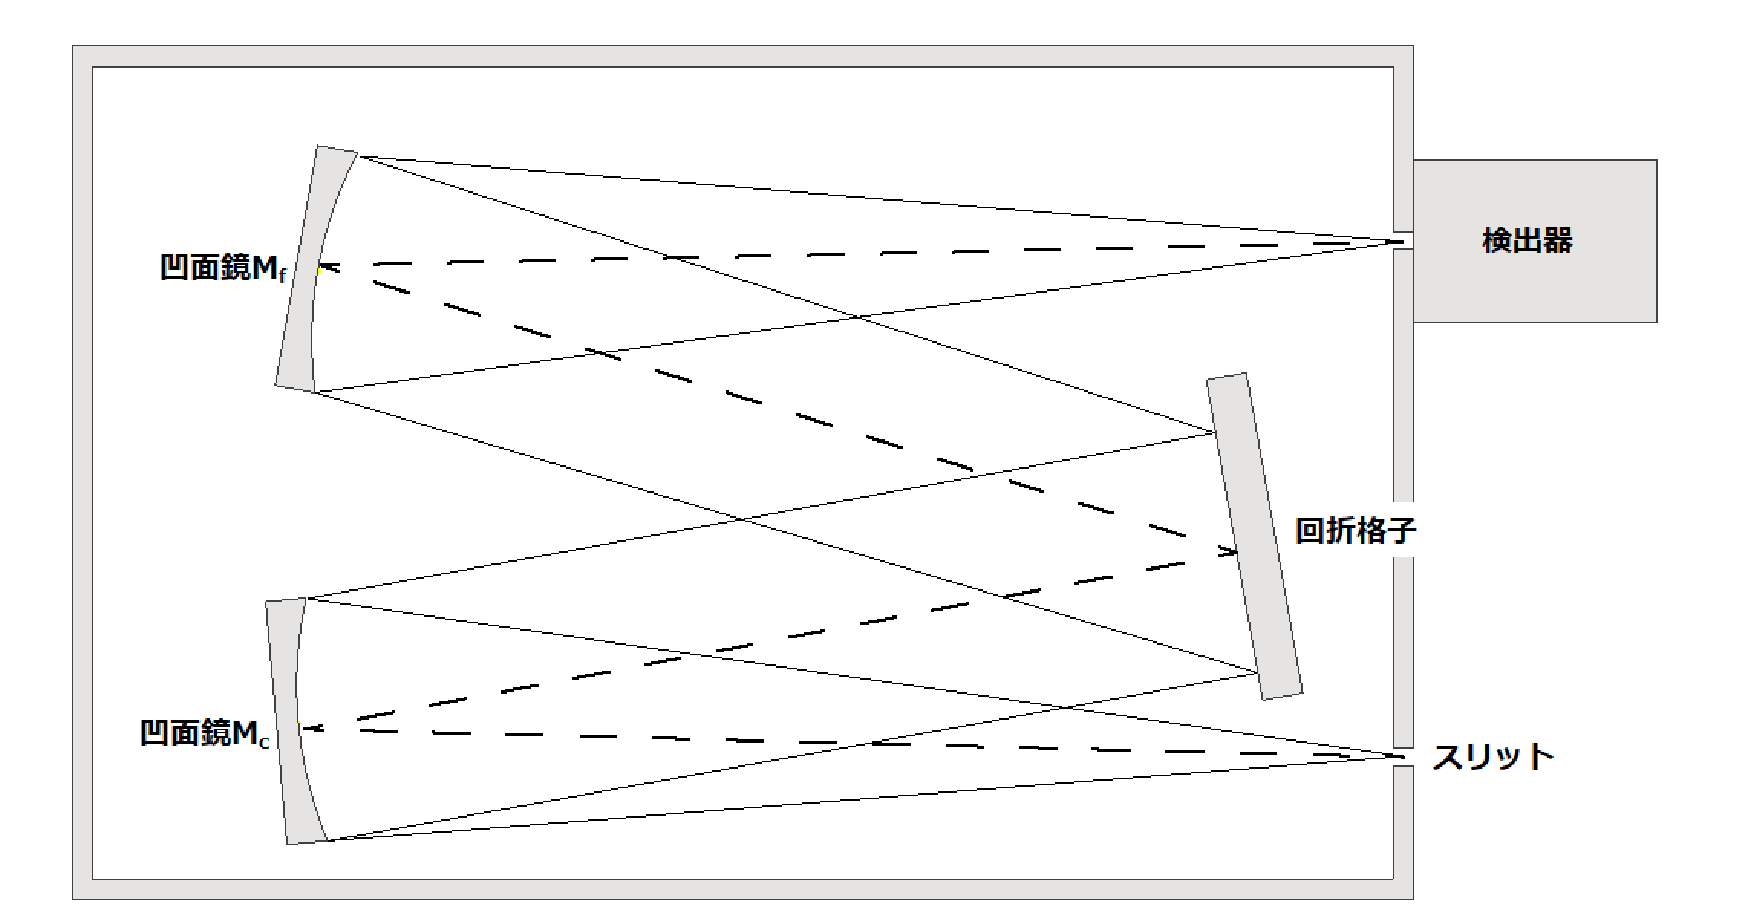
\includegraphics[scale=0.4]{figure/czerny_turner.pdf}
    \caption{ツェルニ・ターナ型分光器の概略図}
    \label{fig:czerny_turner}
\end{figure}
分光器は主にスリット,コリメータ,結像器,回折格子,検出器から構成されている.
ツェルニ・ターナ型分光器ではコリメータ及び結像器には凹面鏡が使用されている.
また,検出器にはCCDカメラやCMOSカメラが用いられている.
この分光器にさまざまな波長の光を入れた場合について考える.
入口スリットから入った光は凹面鏡$\mathrm{M_c}$に反射して平行光となり,回折格子に入射する.
回折格子によって光は波長ごとの異なる角度に回折し,凹面鏡$\mathrm{M_f}$によって検出器受光面に結像される.
この時取り出したい波長以外の光は凹面鏡$\mathrm{M_f}$から外れるか,検出器受光面からずれた位置で集光されている.回折格子の角度を調節することで任意の波長の光を観測することができる\cite{spectrometer}.

% 同じく一般的な分光器であるリトロー型分光器はツェルニ・ターナ型におけるコリメート鏡と結像鏡を共用した構成である.\cite{anritsu}

% 緒言で述べた通りツェルニ・ターナ型分光器は光路内に軸外反射を持つため収差が発生しやすい.
% ここでosloを用いて軸外反射のシミュレーションを行う.
% 軸外反射では特にコマ収差という彗星のように尾を引いてぼやける収差の影響が大きい.
% 球面鏡の軸外反射によってコマ収差が生まれている様子をFig.\ \ref{fig:koma_syuusa}に示す.
% \begin{figure}[htbp]
    % \centering
    % 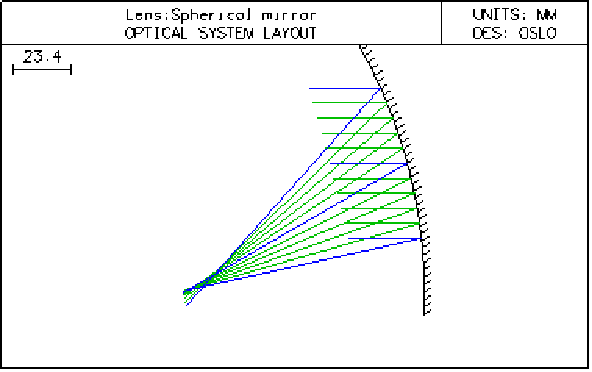
\includegraphics[scale=0.8]{figure/koma_syuusa.pdf}
    % \caption{コマ収差の様子}
    % \label{fig:koma_syuusa}
% \end{figure}
% 緒言で述べた通りツェルニ・ターナ型分光器は光路内に軸外反射を持つため収差が発生しやすい.
% また,軸外反射はより大きな角度で反射するほど収差は大きくなる.

% ツェルニ・ターナ型分光器では二つの凹面鏡を近付けるほど軸外反射の角度を小さくすることができる.
% また同様に凹面鏡から回折格子までの距離を離せば離すほど軸外反射の角度を小さくすることができるが,一般に回折格子が回転するための余裕などを考え凹面鏡と回折格子の距離を凹面鏡の焦点距離の7~8割程度にして配置しているものが多い.
% 例として有効径が100 mm,焦点距離が約1500 mmの球面鏡を用いて球面鏡から回折格子までの距離を焦点距離の8割である1200 mmにすると,二つの球面鏡を可能な限り近づけて配置しても軸外反射の角度は計算上3.6°となる.
% 実際には二つの球面鏡は少し離れて設置されるので軸外反射の角度は4°ほどになると考えられる.


% ここで高度な光線追跡やスポットサイズ解析などを行えるソフトウェアであるOSLOを用いて軸外反射のシミュレーションを行う.
% 球面鏡を結像器として用いた際のスポットの様子を作成した.
% Fig.\ \ref{fig:off_axis_spot_0},Fig.\ \ref{fig:off_axis_spot_1},Fig.\ \ref{fig:off_axis_spot_2}はそれぞれ有効径が100 mm,焦点距離が約1500 mmの球面鏡に対して波長587.6 nmの光を垂直に入射させた際のスポット,軸外反射の角度を2°に設定した際のスポット,軸外反射の角度を4°に設定した際のスポットを表す.
% \begin{figure}[htbp]
%     \centering
%     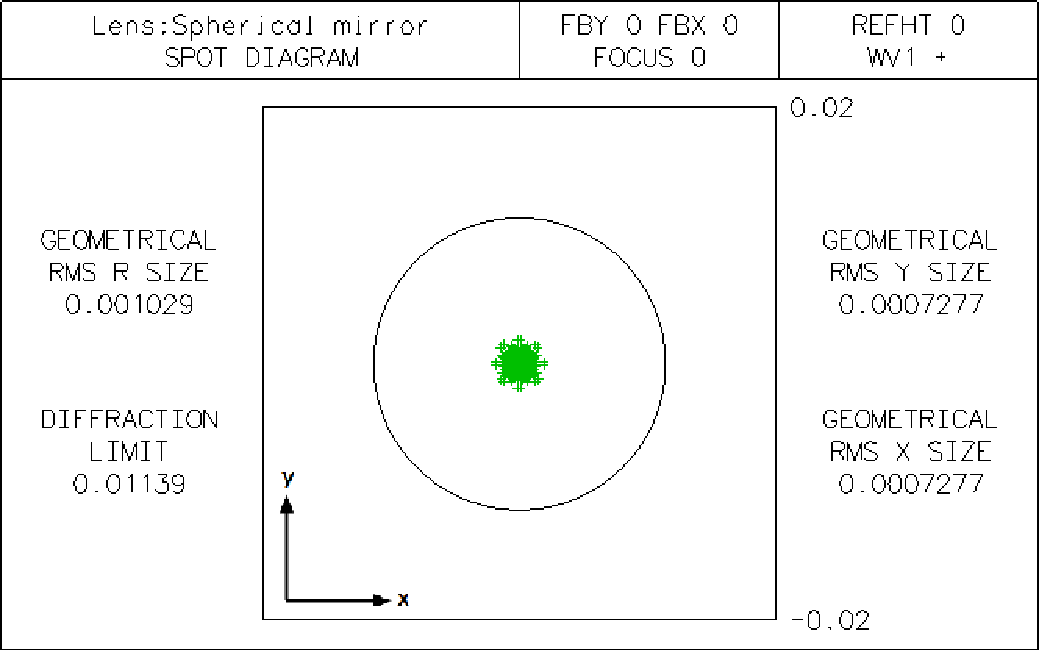
\includegraphics[scale=0.8]{figure/off_axis_spot_0.pdf}
%     \caption{球面鏡で集光した際のスポット(光を垂直に入射)}
%     \label{fig:off_axis_spot_0}
% \end{figure}
% \begin{figure}[htbp]
%     \centering
%     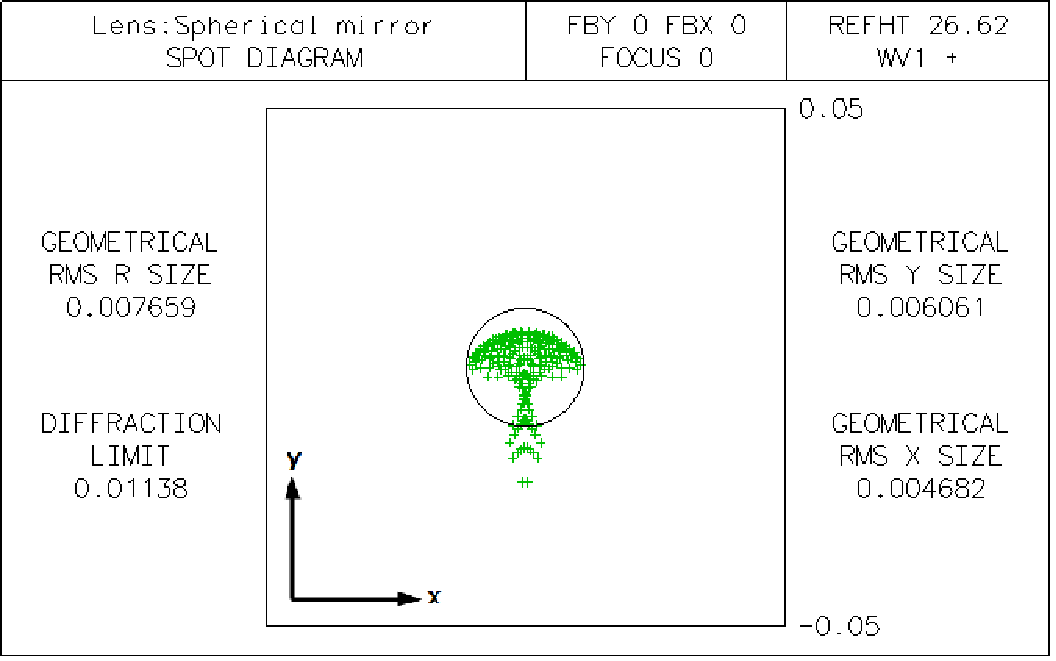
\includegraphics[scale=0.8]{figure/off_axis_spot_1.pdf}
%     \caption{球面鏡で集光した際のスポット(軸外反射の角度を2°に設定)}
%     \label{fig:off_axis_spot_1}
% \end{figure}
% \begin{figure}[htbp]
    % \centering
    % 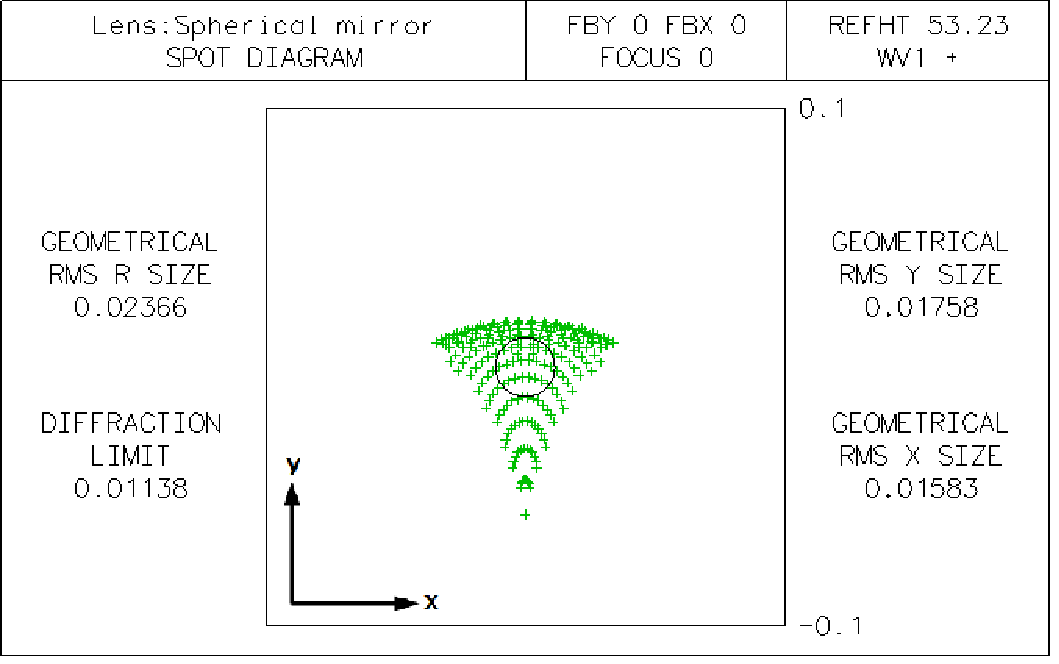
\includegraphics[scale=0.8]{figure/off_axis_spot_2.pdf}
    % \caption{球面鏡で集光した際のスポット(軸外反射の角度を4°に設定)}
    % \label{fig:off_axis_spot_2}
% \end{figure}
% 表示されている数字の単位は全て[mm]である.
% これらの図を見ると軸外反射の角度を大きくするほどスポットが大きくなることがよくわかる.
% 黒い円はエアリーディスクを表しており,Fig.\ \ref{fig:off_axis_spot_0}のようにすべての光線がこの中に収まっている時,回折限界に到達していると言える.
% 対してFig.\ \ref{fig:off_axis_spot_2}のように軸外反射の角度を4°に設定し集光した場合,光はエアリーディスクから大きくはみ出しており,収差の影響を受けることが分かる.
% https://www.an.shimadzu.co.jp/uv/support/lib/uvtalk/uvtalk3/basic.htm


\section{回折格子の基本式}
今回,回折格子が図\ \ref{fig:czerny_turner}のように分光器内で使用されていることを前提に回折格子の基本式について説明を行う.
図\ \ref{fig:grating_principle}に反射型の回折格子による光の回折の様子を模式的に表す.
\begin{figure}[htbp]
    \centering
    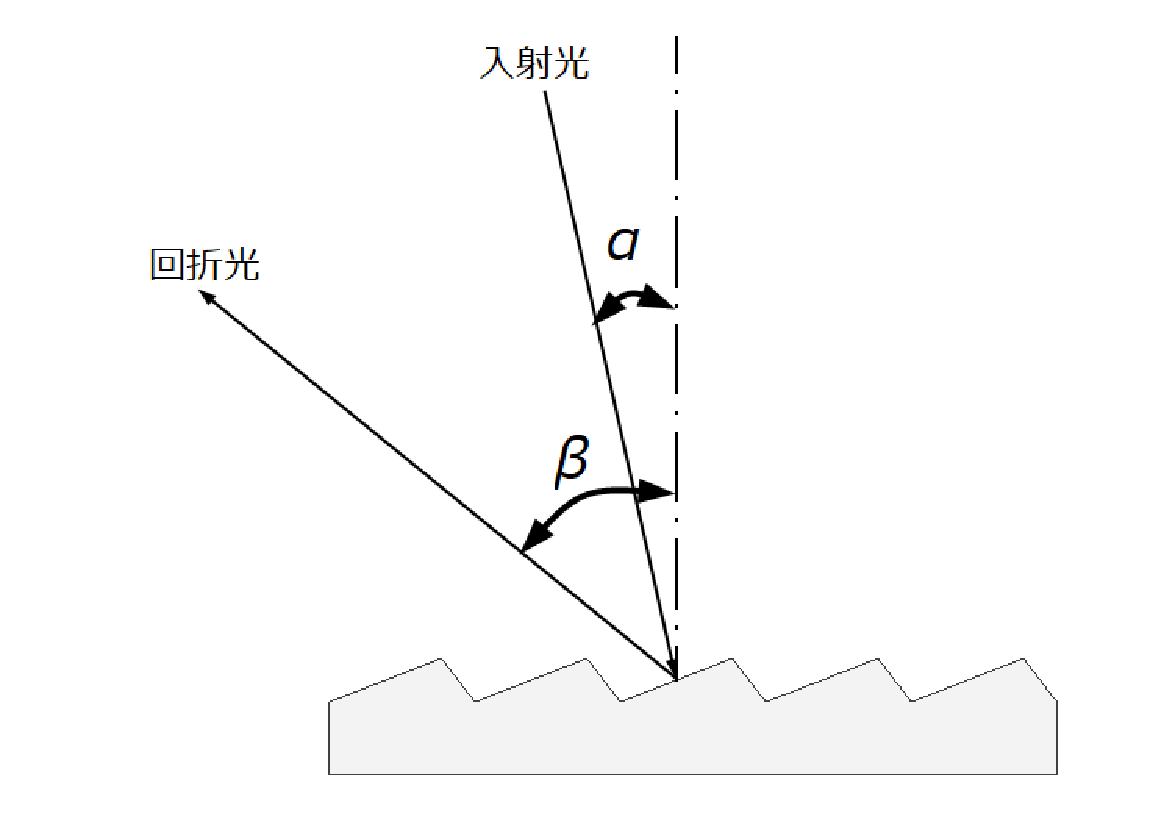
\includegraphics[scale=0.5]{figure/grating_principle.pdf}
    \caption{回折格子における光の回折}
    \label{fig:grating_principle}
\end{figure}
単位長さ当たりの刻線数が$N$の回折格子に波長$\lambda$の光が入射するとき,入射角を$\alpha$,回折角を$\beta$,回折の次数を$m$とすると入射光が回折格子の刻線に垂直な面上にある場合,回折格子の入射角と反射角の関係は以下の式で表される.
\begin{equation}
     Nm\lambda = \mathrm{sin}{\alpha}+\mathrm{sin}{\beta}
\end{equation}
% ここでFig.\ \ref{fig:grating_principle}に示すように入射角と回折角のなす角が$2a$で一定であるとすると,入射角$\alpha$と回折角$\beta$は以下のように表すことができる.
% \begin{eqnarray}
%      \alpha&=&\Phi - a \\
%      \beta&=&\Phi + a
% \end{eqnarray}
% 従って,式(2.1)は
% \begin{eqnarray}
%      Nm\lambda&=&\mathrm{sin}{\alpha}+\mathrm{sin}{\beta} \\
%       &=&2\mathrm{sin}{\frac{\alpha+\beta}{2}}\mathrm{cos}{\frac{\alpha-\beta}{2}}\\
%       &=&2\mathrm{sin}{\Phi}\mathrm{cos}{a}
% \end{eqnarray}
% とできる.
% ここで,$\Phi$は入射角と回折角の二等分線と回折格子の法線がなす角を表す.
% 分光器では$\Phi$を変化させることによって任意の波長を観測することができる.
% レイリーの基準によると,波長$\lambda$のスペクトルの第1極小値の位置に$\lambda+	d\lambda$のスペクトルの最大値がくるときを波長分解の限界と定義している.
% このときの分解能$\lambda/	d\lambda$を理論分解能といい次式で表される.
% \begin{equation}
    %  \frac{\lambda}{d\lambda} = m N W
% \end{equation}
% ここで$W$は回折格子の有効幅であり,$NW$は回折格子に光が当たっている部分の総刻線数を表す.
式(2.1)の両辺を$\lambda$で微分すると,回折格子の角分散($d\beta$/$d\lambda$)が得られる.
なお,角分散は波長に対する回折角の変化量を表す.
\begin{eqnarray}
    \frac{d\beta}{d\lambda} = \frac{Nm}{\mathrm{cos}{\beta}}
\end{eqnarray}
逆線分散は検出器結像面上において単位長さ離れた位置での波長差を表す.
結像器の焦点距離を$f$として,回折角が$d\beta$だけ変化したとき,結像位置が$dx=fd\beta$ずれることから,逆線分散($d\lambda$/$dx$)は次式で表される.
\begin{eqnarray}
    \frac{d\lambda}{dx} = \frac{\mathrm{cos}{\beta}}{Nmf}
\end{eqnarray}
この逆線分散に検出器の受光面の長さを掛けると一度に測定できる波長範囲になる.

回折光の拡大率は分光器において検出器受光面に入射スリットの像が結像される際の像の大きさの倍率を表す.
拡大率($d\alpha$/$d\beta$)は式(2.1)で$\lambda$を一定と置き,両辺を$\beta$で微分すると得られる.
\begin{eqnarray}
    \frac{d\alpha}{d\beta} = -\frac{\mathrm{cos}{\beta}}{\mathrm{cos}{\alpha}}
\end{eqnarray}
スリット幅に拡大率の絶対値($|d\alpha$/$d\beta|$)と逆線分散($d\lambda$/$dx$)を掛け合わせると,スリット幅が有限であることに起因するスペクトルの波長幅になる.
スリット幅を$s$としたとき,この波長幅($d\lambda$)は
\begin{eqnarray}
     d\lambda &=& s\left|\frac{d\alpha}{d\beta}\right|\frac{d\lambda}{dx} \nonumber \\%
        &=&s\frac{\mathrm{cos}{\beta}}{\mathrm{cos}{\alpha}}\frac{\mathrm{cos}{\beta}}{Nmf} \nonumber \\
        &=&\frac{s\mathrm{cos}^2{\beta}}{Nmf\mathrm{cos}{\alpha}}
\end{eqnarray}
と表される.

\section{CCDカメラ}
\subsection{動作原理}
% CCDカメラとはCCDイメージセンサという半導体素子が搭載された高感度のカメラである.
% CCDイメージセンサは光の強さに応じた電荷を出し,電気信号に変換する.
CCDとはCharge Coupled Deviceの略であり,日本語では電荷結合素子と表される光の強さを電気信号に変換する半導体素子である.
CCDは格子状に並んだピクセルから構成されている.
各ピクセルの受光部(フォトダイオード)に光が当たると光の強さに応じた電荷が発生し蓄積される\cite{ccd}.
ここで蓄積された電荷を1ピクセルずつ順次転送して最終的に各画素の電荷を電荷電圧変換アンプで電圧に変換して読み取る\cite{ccd_principle}.
% CCDは光の強さに応じた電荷を出し,その電荷を次々と転送することによって電気信号に変換する半導体のことである.

% CCDにおける電荷転送はよくバケツリレーに例えられるように各ピクセルの持っている信号電荷を隣のピクセルに移すという動作を繰り返すことによって成り立っている.
% 端まで転送された信号電荷は順に電気信号として出力される\cite{ccd}.
% https://www.hamamatsu.com/resources/pdf/ssd/ccd_kmpd9002j.pdf

% https://www.jstage.jst.go.jp/article/itej/68/2/68_145/_pdf

\subsection{ビニング}
CCDでは複数の隣接するピクセルの信号電荷を加算し一つのピクセルとして出力することが可能である.
この動作をビニングと呼ぶ.
ここで,ビニングしたピクセルの数をビニングサイズと呼ぶこととする.
ビニングを行うと解像度が低下する.
一方,ビニングを行うと読み出し回数が減るため読み出しノイズが減少し読み出しスピードが速くなる.
S/N比が良くなるため,微弱な光を読み取る場合にはビニングは有効である.




% https://www.jstage.jst.go.jp/article/lsj/39/10/39_780/_pdf